\documentclass[10pt]{standalone}
\usepackage{tikz}

% TikZ libraries `calc` needed now to tweak bracket.
\usetikzlibrary{backgrounds,fit,decorations.pathreplacing,calc}
% Dirac Kets
\newcommand{\ketone}[1]{\ensuremath{\left|#1\right\rangle^{\otimes nd}}}

\newcommand{\kettwo}[1]{\ensuremath{\left|#1\right\rangle^{\otimes n_0}}}

\newcommand{\ket}[1]{\ensuremath{\left|#1\right\rangle}}

\begin{document}
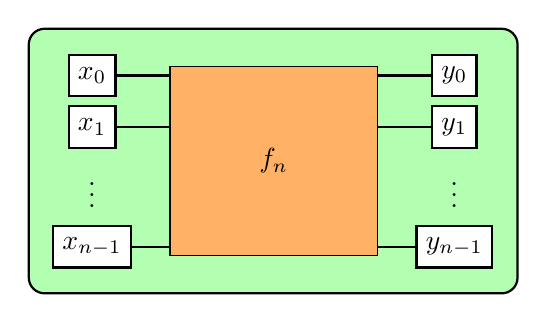
\begin{tikzpicture}[thick]
	% `phase' is used for controlled phase gates (dots).
	% `surround' is used for the background box.
	\tikzstyle{bit} = [draw,fill=white,minimum size=1.5em] 
	\tikzstyle{Roperator} = [draw,fill=purple!60!white,minimum size=1.5em] 
	\tikzstyle{computer} = [draw,fill=orange!60!white,minimum size=1.5em] 
	\tikzstyle{phase} = [draw,fill,shape=circle,minimum size=5pt,inner sep=0pt]
	\tikzstyle{surround} = [fill=green!30,thick,draw=black,rounded corners=2mm]
	\tikzstyle{blank} = [fill=green!30]
	%\tikzset{oldmeter/.append style={draw, inner sep=10, rectangle, font=\vphantom{A}, minimum width=30, line width=.8, path picture={\draw[black] ([shift={(.1,.3)}]path picture bounding box.south west) to[bend left=50] ([shift={(-.1,.3)}]path picture bounding box.south east);\draw[black,-latex] ([shift={(0,.1)}]path picture bounding box.south) -- ([shift={(.3,-.1)}]path picture bounding box.north);}}}
	 \tikzset{meter/.append style={draw, fill=white, inner sep=10, rectangle, minimum width=10pt,
	 path picture={\draw[black] (
 	[shift={(.1,.2)}]path picture bounding box.south west) to[bend left=40] %offset from bottom left corner
	([shift={(0,.1)}]path picture bounding box.center) to [bend left = 45] %To just offset from center
	([shift={(-.1,.2)}]path picture bounding box.south east) %To offset from bottom right of box
	;\draw[black,-latex] ([shift={(0,.2)}]path picture bounding box.south) -- ([shift={(.3,-.1)}]path picture bounding box.north);}]}} % Draw the arrow
	%
	\matrix[row sep=0.1cm, column sep=0.6cm] (circuit) {
	% First row.
		\node[bit] (x00) {$x_0$}; &
			\coordinate (comp00);&&&
		\coordinate (comp01);&
		\coordinate (x02);&
		\node[bit] (y0) {$y_0$};
		\\
	% second row.
		\node[bit] (x10) {$x_1$}; &
			\coordinate (comp10);&&&
		\coordinate (comp11);&
		\coordinate (x12);&
		\node[bit] (y1) {$y_1$};
		\\
	%ellipsis
		\node (ellx) {$\vdots$}; &
			\coordinate (ell2);&&&
		\coordinate (ell3);&
		\coordinate (ell4);&
		\node (elly) {$\vdots$};
		\\
	% last row.
		\node[bit] (xn0) {$x_{n-1}$}; &
			\coordinate (compn0);&&&
		\coordinate (compn1);&
		\coordinate (xn2);&
		\node[bit] (yn) {$y_{n-1}$};
		\\
		};
	% Draw bracket on right with resultant state.
		%\node[rectangle, draw, fill=white, minimum width = 1.5em, minimum height = 1.65cm][fit = (q17) (q27)] (box) {};
		%\node[align=center] at (box.center){A};
	\begin{pgfonlayer}{background}
		% Draw background box.
		\node at([xshift=-1.6em,yshift= 1em]x00) (corner1) {};
		\node at([xshift= 1.6em,yshift=-1em]yn) (corner2) {};
		\node[surround] (background) [fit = (corner1) (corner2)] {};
		% Draw lines.
		\draw[thick] (x00) -- (y0) ;
		\draw[thick] (x10) -- (y1) ;
		\draw[thick] (xn0) -- (yn) ;
		%\draw[thick] ([yshift=-5pt]5.5, 0.6725) -- ([yshift=-1pt]end1) ;
		%\draw[thick] ([yshift=-5pt]5.5, 0.740) -- ([yshift=1pt]end1) ;
		%
		%\draw[thick] ([yshift=1pt] meter1 |- 5.5, 1 |- end1) -- ([yshift=1pt]end1) ;
		%\draw[thick] ([yshift=-1pt] meter1 |- 5.5, 1 |- end1) -- ([yshift=-1pt]end1) ;
		%
		%
		%\node[blank] at (q23) (background) {\ldots};
		%\node[blank] at (q27) (background) {\ldots};
		%\node[blank] at (q210) (background) {\ldots};
		%\node at ([yshift=-1.5em]q210) (psi4) {\ket{\ensuremath{\psi_4}}};
		%\draw[->, >=stealth] (q111) -- (psi4);
		\node[computer] (computer) [centered, fit = (comp00) (xn2)] {};
		\node at (computer) {$f_n$};
	\end{pgfonlayer}
%
\end{tikzpicture}
\end{document}
